\newacronym{api}{API}{Application Programming Interface}

\section{Evaluation Comparison}\label{sec:result_comparison}
In the final evaluation step we take a broader look on the overall performance. For that, we combined the results from each dataset. This has the advantage of reducing the sensibility to a particular dataset which is required to keep bias at minimum. 

Based on our initial hypothesis which motivates Context enrichment, we have formulated a couple of questions that were answered in the next paragraphs:
\paragraph{Which Context enrichment method performed best in general?}
Our observations confirmed our initial hypothesis which suggests extending basic crowd-based ontology validation with Context. From the combined results of all datasets as shown in~\hyperref[table:bench_p_r_f_combined]{Table~\ref*{table:bench_p_r_f_combined}} it is evident that Embedded~Context worked best. In fact, it had not only the highest value of F-Measure but also the highest Precision and Recall. Indeed, this was rather expected due to the fact that Context was manually added. Obviously, no one has a better domain knowledge than the creators or maintainers of the ontology. 
On the bottom end of the table is the previous approach without descriptions. 
\begingroup
\renewcommand{\arraystretch}{1.5}
\begin{table}
	\begin{tabularx}{\textwidth}{l c*{3}{Y}}
		\toprule
		Method & Precision & Recall & F-Measure \\
		\midrule
		 Embedded Context & 0.797 & 0.921 & 0.854 \\
		 Neighbouring Nodes & 0.787 & 0.887 & 0.834 \\
		 External Source & 0.729 & 0.899 & 0.805 \\
		 None & 0.674 & 0.910 & 0.775 \\
		\bottomrule
	\end{tabularx}
	\caption{Aggregated results of all datasets~(ranked by F-Measure)}
	\label{table:bench_p_r_f_combined}
\end{table}
\endgroup

\paragraph{Did the crowd perform better with Context?}
\hyperref[fig:results_accuracy_combined]{Figure~\ref*{fig:results_accuracy_combined}} depicts the combined accuracy of all methods which is calculated
as the ratio between correct and incorrect judgements. For comparability, the exact number of judgements were written in labels. The performance of the top ranked method~(Embedded Context) is quite impressive. Concepts were judged correctly for nearly eighty percent~($78.4\%$), being an improvement of over $14\%$ compared to omitting concept descriptions. Even the last ranked enrichment method~(External Source), performs $4.6\%$ better.
\begin{figure}
	 \centering
	 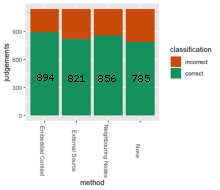
\includegraphics[width=0.75\textwidth]{plots/comparison/barplot_all_judgements}
	 \caption{Combined accuracy of Crowdsourcing methods}\label{fig:results_accuracy_combined}
\end{figure}

\paragraph{For which concepts were the crowd wrong?}
Even though the results underlined the usefulness of Context for crowd-sourced ontology validation, we were also interested under which circumstances they failed. In particular, we evaluated for which concepts the crowd had the most problems with. The goal was to identify common patterns to guide future improvements. 

\hyperref[table:combined_evaluation_bad_concepts]{Table~\ref*{table:combined_evaluation_bad_concepts}} lists 6 concepts that had the highest number of erroneous judgements. The concept \emph{sceptic} is located in the top-most row of the table. None of the judgements were correct for that concept. 
Consequently, for the climate change ontology, the concept was rejected even with Context being present. An explanation for that could be the fact
the Context was too generic or inappropriate. Clearly, the concept could be associated with climate change, meaning someone who doubts global warming.
Unfortunately, we were not able to adapt Context because we had no access to the sources where the ontologies were learned from. 
In most cases though, we expect ontology engineers to have enough knowledge to provide more accurate descriptions that were useful to the crowd.
\begingroup
\renewcommand{\arraystretch}{1.5}
\begin{table}
	\begin{tabularx}{\textwidth}{l c*{4}{Y}}
		\toprule
		\multirow{2}{*}{\emph{Concept}} & \multicolumn{4}{c}{\emph{Methods}} & \emph{Accuracy}\\
		\cmidrule(lr){2-5} \cmidrule(lr){6-6} 
		 & EC & NN & ES & NONE & Total\\
		\midrule
		sceptic & 0/5 & 0/5 & 0/5 & 0/5 & 0/20 \\
		greenhouse & 0/5 & 1/5 & 0/5 & 0/5 & 1/20 \\
		pipeline & 0/5 & 0/5 & 1/5 & 0/5 & 1/20 \\
		consensus & 2/5 & 0/5 & 0/5 & 0/5 & 2/20 \\
		denier & 2/5 & 0/5 & 0/5 & 0/5 & 2/20 \\
		production & 1/5 & 1/5 & 0/5 & 0/5 & 2/20 \\
		\bottomrule
	\end{tabularx}
	\caption{Concepts where most crowd workers had problems~(EC=Embedded Context, NN=Neighbouring Nodes, ES=External Source, NONE=No Context)}
	\label{table:combined_evaluation_bad_concepts}
\end{table}
\endgroup

For the remaining concepts the situation is similar. We identified the following pattern: Context was either missing, especially for very specific concepts, or too generic. The only solution to both is strengthen collaboration between ontology engineers and domain experts. 

\paragraph{What other issues were found?}
A general phenomenon of all approaches was the relatively high value of Precision indicating that the crowd tends to rather reject concepts in case 
of uncertainty or lack of knowledge. However, in ontology engineering Recall is often more important than Precision. Domain experts and ontology maintainers prefer deleting a few concepts rather than missing some important ones. 

Another observation was that not all enrichment methods worked in all scenarios.
For some concepts~($17\%$) no Context was found when fetching from the online dictionary WordNik. Most of these concepts had names that were composed of multiple words as it was the case for \emph{interest rate}. Compound words were treated as if words were searched separately. The final result then being merged from each subquery. Unfortunately, the \gls{api} does not support changing this behaviour to treat compound words as a whole. 

The number of concepts with missing Context was quite low when descriptions were generated from the ontology structure. For $30\%$ of the concepts Context was missing. Obviously, the algorithm failed when the concept was not part of a subsumption relation. In such situations, other approaches that do not rely on the ontology structure should be used instead. 

Strangely, Context was not always helpful, in certain situations it can also be distracting, mainly if it provides useless or even misleading information. Regrettably, some content fetched from WordNik was rather lengthy or diffuse. That was certainly due to the fact that content originated from blogs or tweets that were not well suited for word definitions. Future versions of the framework could try to use a different content provider which provides more concise information.
